\documentclass[12pt]{article}
\usepackage{preamble}

\pagestyle{fancy}
\fancyhead[LO,LE]{Дополнительные главы \\ высшей математики}
\fancyhead[RO,RE]{Лекции Далевской О. П.}

\fancyfoot[L]{\scriptsize исходники найдутся тут: \\ \url{https://github.com/pelmesh619/itmo_conspects} \Cat}

\renewcommand{\thesection}{}

\begin{document}

    \tableofcontents
    \clearpage

    % begin addchapters2_2025_02_07.tex





\section{1. Основные понятия}

\subsection{1.1. Комплексное число}

\Mem $\Complex = \{ (a, b) \ | \ a, b \in \Real\}$

Обозначение: $z = (a, b) = a + bi$, где $i = (0, -1) = \sqrt{-1}$

\underline{Основные операции}:

\begin{enumerate}
    \item $\RE z = a$ - вещественная часть, $\IM z = b$ - мнимая часть
    \item $z_1 + z_2 = (a_1, b_1) + (a_2, b_2) = (a_1 + a_2, b_1 + b_2) = (a_1 + a_2) + i(b_1 + b_2)$
    \item $z_1 \cdot z_2 = (a_1 + b_1 i) * (a_2 + b_2 i) = (a_1 a_2 - b_1 b_2) + i (a_1 b_2 + a_2 b_1)$
    \item $z^n = \rho^n (\cos n\varphi + i \sin n\varphi)$ - \textbf{формула Муавра}, где $\rho = |z|, \varphi = \arg z$
    \item $\sqrt[n]{z} = \sqrt[n]{\rho} \left(\cos \frac{\varphi + 2\pi k}{n} + i \sin \frac{\varphi + 2\pi k}{n}\right)$, где $\rho = |z|, \varphi = \arg z, k \in \Integer$
    \item При $n = 2$ $\sqrt{z} = \sqrt{a + bi} = \pm (c + di)$, 
        где $c = \sqrt{\frac{a + \sqrt{a^2 + b^2}}{2}}, d = \operatorname{sign}(b) \sqrt{\frac{-a + \sqrt{a^2 + b^2}}{2}}$
\end{enumerate}

\begin{minipage}{\textwidth}
    % https://www.geogebra.org/calculator/xjg67fnv

    \begin{wrapfigure}{r}{0pt}
        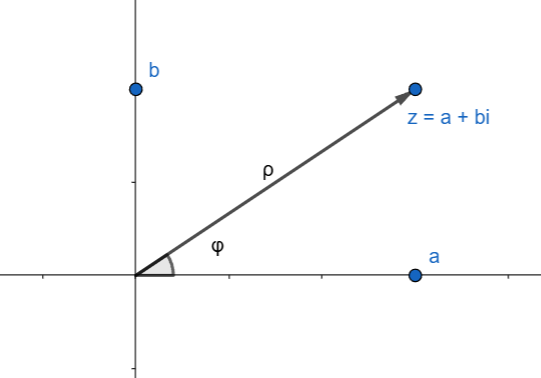
\includegraphics[width=7cm]{addchapters2/images/addchapters2_2025_02_07_6}
    \end{wrapfigure}

    Тригонометрическая форма:

    $z = a + bi = \rho (\cos \varphi + i \sin \varphi)$, где $\rho = |z| = \sqrt{a^2 + b^2}, \varphi = \arg z \in [0; 2\pi)$

    $\Arg z = \arg z + 2\pi k, k \in \Integer$

    По формуле Эйлера $z = \rho (\cos \varphi + i \sin \varphi) = \rho e^{i \varphi}$
\end{minipage}

\subsection{1.2. Комплексная плоскость}

\Def Окрестность точки $z_0 \in \Complex$ определяется как $U_\delta (z_0) = \{z \in \Complex \ \Big| \ |z - z_0| < \delta\}$

Тогда $\overset{\circ}{U}_\delta (z_0) = U_\delta (z_0) \setminus \{ z_0 \}$ - выколотая окрестность

\Def Для данной множества точек $A$ точка $z_0$ считается

\begin{itemize}
    \item внутренней, если для любого $\delta$ $U_\delta (z_0) \subset A$
    \item граничной, если для любого $\delta$ $\exists z \in U_\delta (z_0) \Big| z \in A$ и $\exists z \in U_\delta (z_0) \Big| z \notin A$
\end{itemize}

\Def Открытое множество состоит только из внутренних точек

\Defs Закрытое множество содержит все свои граничные точки

\Defs Границой $\Gamma_D$ (иногда обозн. $\delta D$) для множества $D$ называют множество всех граничных точек $D$

\Defs Если любые две точки множества можно соединить ломаной линией конечной длины, то множество считается связным

\Defs Множество $D \subset \Complex$ называется областью, если $D$ - открытая и связная

\Defs Кривая $l \subset \Complex$ считается непрерывной, если $l = \{z \in \Complex \ | \ z = \varphi(t) + i \psi(t), t \in \Real\}$, где $\varphi(t), \psi(t)$ - непрерывные функции

\Notas Если $\varphi(t)$ и $\psi(t)$ дифференцируемы и их производные непрерывные, то кривая $l$ гладкая

\Defs Непрерывная замкнутая (то есть начальная и конечная точки совпадают) без самопересечений кривая называется контуром

\Notas Односвязную область можно стянуть в точку

% https://www.geogebra.org/calculator/nhbjhbag

\begin{multicols}{2}
    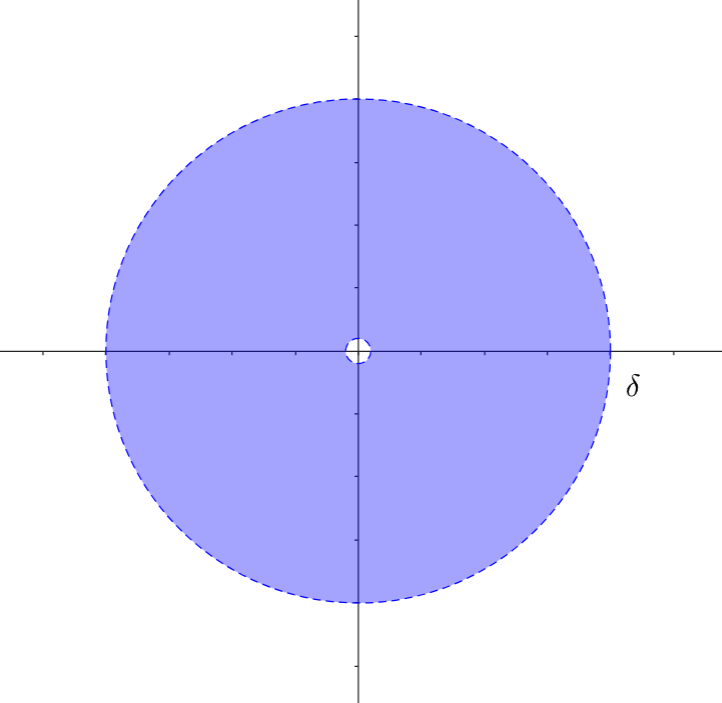
\includegraphics[width=0.4\textwidth]{addchapters2/images/addchapters2_2025_02_07_1}

    \ExNs{1} $D = \{z \in \Complex \ \Big| \ 0 < |z| < \delta\}$ - область связаная, но не односвязная, ее нельзя стянуть из-за дырки

    \mediumvspace

    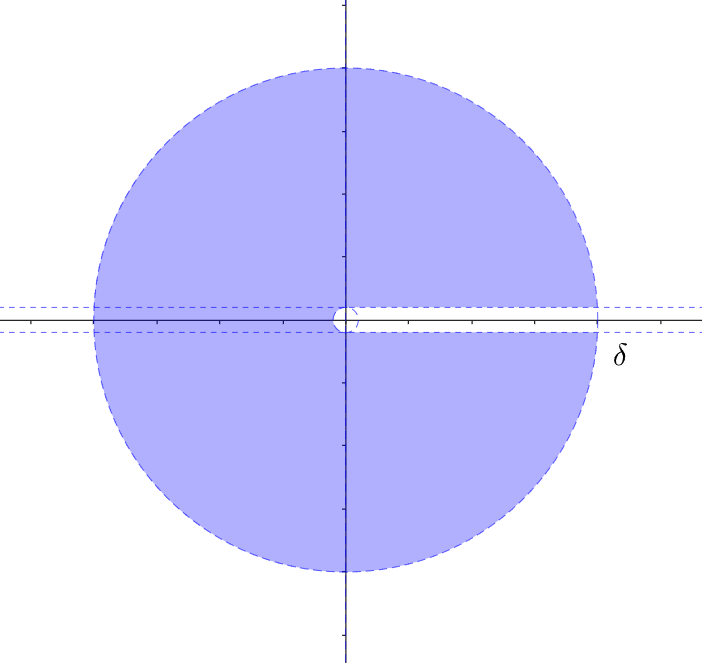
\includegraphics[width=0.4\textwidth]{addchapters2/images/addchapters2_2025_02_07_2}

    \ExN{2} $D = \{z \in \Complex \ \Big| \ 0 < |z| < \delta, \arg z \neq 0\}$ - область связная и односвязная
\end{multicols}

\begin{multicols}{2}
    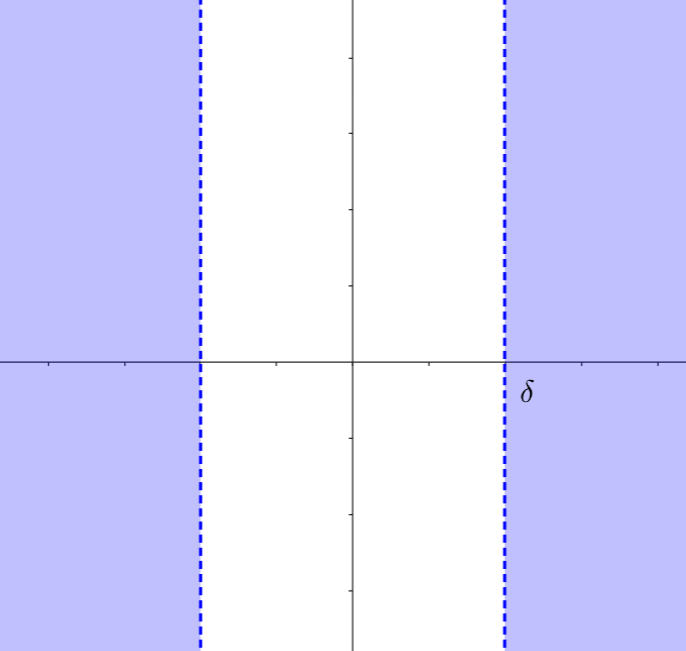
\includegraphics[width=0.4\textwidth]{addchapters2/images/addchapters2_2025_02_07_3}

    \ExN{3} $D = \{z \in \Complex \ \Big| \ |\RE z| < \delta\}$ - несвязная область

    \mediumvspace

    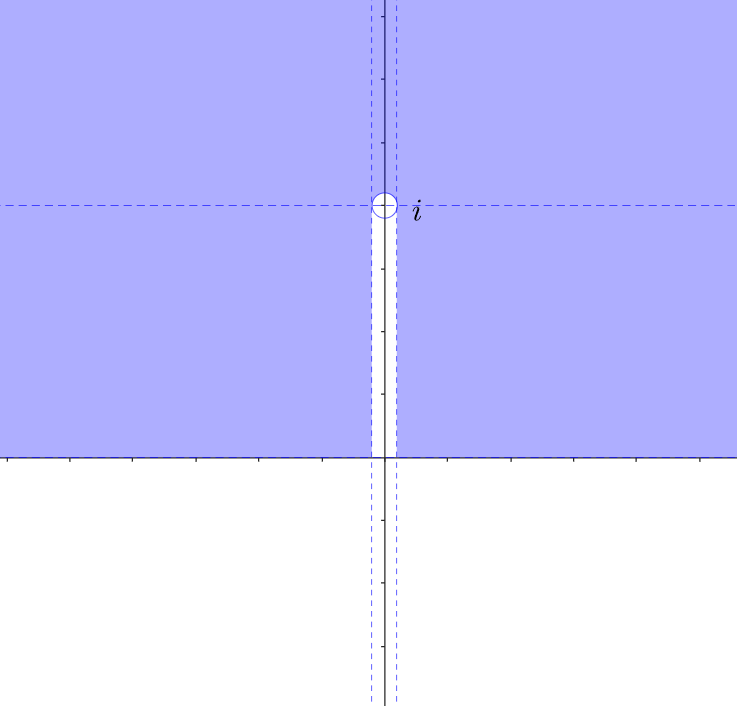
\includegraphics[width=0.4\textwidth]{addchapters2/images/addchapters2_2025_02_07_4}

    \ExN{4} $D = \{z \in \Complex \ \Big| \ \IM z \geq 0, z \notin [0, i]\}$ - здесь под $[0, i]$ подразумевается линейный отрезок на оси
\end{multicols}

\Nota Дальше все рассматриваемые $\Gamma_D$ будут состоять из кусочногладких и изолированных кривых

\subsection{1.3. Предел}

\Mem Последовательность $\{z_n\} = z_1, z_2, z_3, \dots, z_n, \dots$

\Def Пределом $\{z_n\}$ называют число $z$ такое, что

$\forall \varepsilon > 0 \ \exists \underset{n_0 = n_0(\varepsilon)}{n_0 = \Natural} \ \Big| \ \forall n > n_0 \ |z_n - z| < \varepsilon$

Обозначается $\lim_{n \to \infty} z_n = z$

\Nota $\{z_n\}$ можно представить как ${x_n + i y_n}$, то есть двумя $\Real$-последовательностями

\begin{MyTheorem}
    \Ths $\exists \lim_{n \to \infty} z_n = \underset{x, y \in \Real}{x + i y} \Longleftrightarrow $
    \begin{tabular}{l} $\exists \lim_{n \to \infty} x_n = \lim_{n \to \infty} \RE z_n = x$ \\ $\exists \lim_{n \to \infty} y_n = \lim_{n \to \infty} \IM z_n = y$ \end{tabular}
\end{MyTheorem}

\begin{MyProof}
    \fbox{$\Longleftarrow$} $\forall \varepsilon > 0 \ \exists \underset{n_0 = \max (n_{0x}, n_{0y})}{n_0 \in \Natural} \ \Big| \ \forall n > n_0 \begin{tabular}{l} |x_n - x| < \frac{\varepsilon}{2} \\ |y_n - y| < \frac{\varepsilon}{2} \end{tabular}$
    
    $|z_n - z| = |(x_n - x) + i(y_n - y)| \leq |x_n - x| + |y_n - y| < \frac{\varepsilon}{2} + \frac{\varepsilon}{2}$

    То есть $\forall \varepsilon > 0 \dots |z_n - z| < \varepsilon$

    \fbox{$\Longrightarrow$} $\forall \varepsilon > 0 \ |z_n - z| = |(x_n - x) + i(y_n - y)| < \varepsilon \Longrightarrow 
    \begin{cases}
        |x_n - x| \leq |(x_n - x) + i(y_n - y)| < \varepsilon \\
        |y_n - y| \leq |(x_n - x) + i(y_n - y)| < \varepsilon \\
    \end{cases} \Longrightarrow \exists \lim_{n \to \infty} x_n = x$ и $\exists \lim_{n \to \infty} y_n = y$

\end{MyProof}

\Nota Для комплексных чисел работают теоремы для пределов (сумма пределов, произведение пределов и т.д.), критерий Коши и другие

\Def $\lim_{n \to \infty} z_n = \infty \Longleftrightarrow \forall \varepsilon > 0 \ \exists \underset{n_0 = n_0(\varepsilon)}{n_0 \in \Natural} \ \Big| \ n > n_0 \ |z| > \varepsilon$

\Defs Точка $z$, определенная как предел, равный $\infty$, называется бесконечно удаленной. Но существует множество последовательностей, чьи пределы удаляются на бесконечность разными путями на плоскости

\Def Стереографическая проекция (сфера Римана)

% https://www.geogebra.org/calculator/kjesw2gx

\begin{center}
    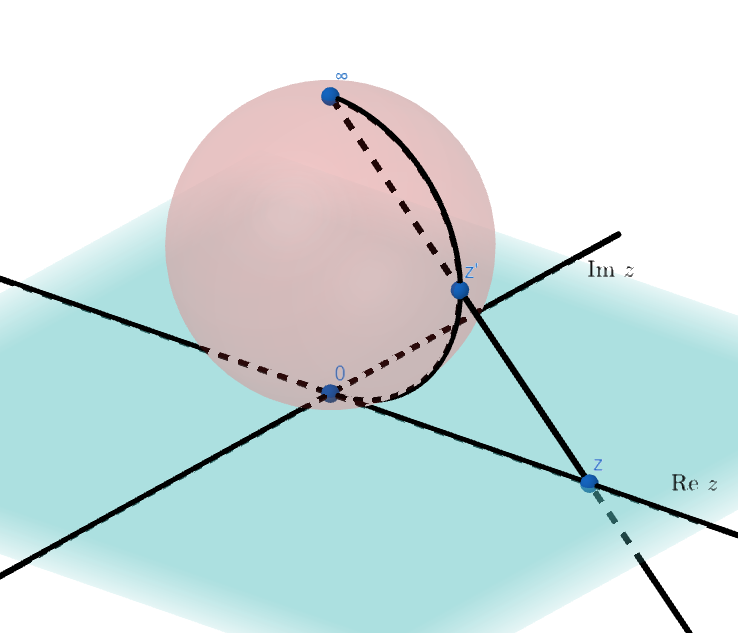
\includegraphics[width=0.55\textwidth]{addchapters2/images/addchapters2_2025_02_07_5}
\end{center}

Поместим сферу на комплексную плоскость и сделаем биекцию точек плоскости на точки сферы: проведем из верхней точки сферы лучи вниз на плоскость, и точка, где луч пересекает сфера,
будет считаться отображением для данной точки. Заметим, что в этом случае бесконечно удаленные точки будут отображаться в верхнюю точку сферы

\Def $\Complex \cup \{\infty\} = \overline{\Complex}$ - расширенная комплексная плоскость

Однако $z + \infty$ не определена, $\infty + \infty$ не определена. 
Но $\infty = \lim_{n \to \infty} \frac{1}{z_n}$ при $z_n \underset{n \to \infty}{\longrightarrow} 0$; $\infty = \infty \cdot \lim_{n \to \infty} z_n$ при $z_n \longrightarrow z$

Записью $[-\infty; +\infty]$ обозначается ось $\overline{\Real}$; 

\qquad\qquad $[-i\infty; +i\infty]$ - мнимая расширенная ось

Путь $x \pm i \infty$ при фикс. $x$ - вертикальная прямая; 

\qquad\qquad $iy \pm \infty$ - горизонтальная прямая; 

\qquad\qquad $e^{i\varphi} \cdot \infty$ - прямая, проходящая через начало координат



% end addchapters2_2025_02_07.tex

% begin addchapters2_2025_02_21.tex





\subsection{1.4. Комплексная функция}

\subsubsection{1$^\circ$ Определение}

\Mem $f : E \subset \Real \longrightarrow D \subset \Real \ \overset{def}{\Longleftrightarrow} \ $ отображение такое, 
что $\forall x \in E \ \exists! y \in D \ | \ y = f(x)$

\Def $f : D \subset \Complex \longrightarrow G \subset \Complex \ \overset{def}{\Longleftrightarrow} \ $ отображение такое, 
что $\forall z \in D \ \exists w \in G \ | \ f(z) = w$

\Defs Если $\forall z \in D \ \exists! w \in G$, то $f$ называется однозначной функцией

\Defs Если $\forall z_1, z_2 \in D (z_1 \neq z_2) \Longrightarrow f(z_1) \neq f(z_2)$, 
то $f$ называется однолистной функцией

\ExN{1} $w = \sqrt{z}$ - неоднозначная функция

$\letsymbol z = 1 = 1 (\cos 0 + i \sin 0)$

$\sqrt{z} = \sqrt{1} \left(\cos \frac{2\pi k}{2} + i \sin \frac{2\pi k}{2}\right)$

$w_1 = 1, \quad w_2 = -1$

\ExN{2} $w = z^2$ - неоднолистная функция

$z_1 = 1, z_2 = -1 \qquad\qquad w(z_1) = w(z_2) = 1$

\Nota Если $f(z)$ однозначна и однолистна, то $f(z)$ - взаимно однозначное соответствие (биекция). Тогда $\exists g(x) \ | \ g(f(x)) = x$

Комплексную функцию $f(z)$ можно представить как $u(x, y) + i v(x, y)$, где $x + iy = z$

\Ex $w = z^2 = (x + iy)^2 = x^2 + 2ixy - y^2 = (x^2 - y^2) + i \cdot 2xy$

$u(x, y) = (x^2 - y^2), \qquad\qquad v(x, y) = 2xy$

\subsubsection{2$^\circ$ Предел}

\Def $L \in \Complex, f : D \longrightarrow G, \quad L \overset{def}{=} \lim_{z \to z_0} f(z) \Longrightarrow
\forall \varepsilon > 0 \ \exists \underset{\delta = \delta(\varepsilon)}{\delta > 0} \ \Big| \ z \in D, z \in \overset{\circ}{U}_\delta(z_0) \ f(x) \in U_\varepsilon(L)$

В определении существование и значение $L$ не должно зависеть от пути, по которому $z$ приближается к точке сгущения $z_0$.
Может быть так, что для любого направления стремления предел есть, но в общем смысле не существует

% https://www.geogebra.org/calculator/hgk25mjs

\begin{wrapfigure}{R}{0pt}
    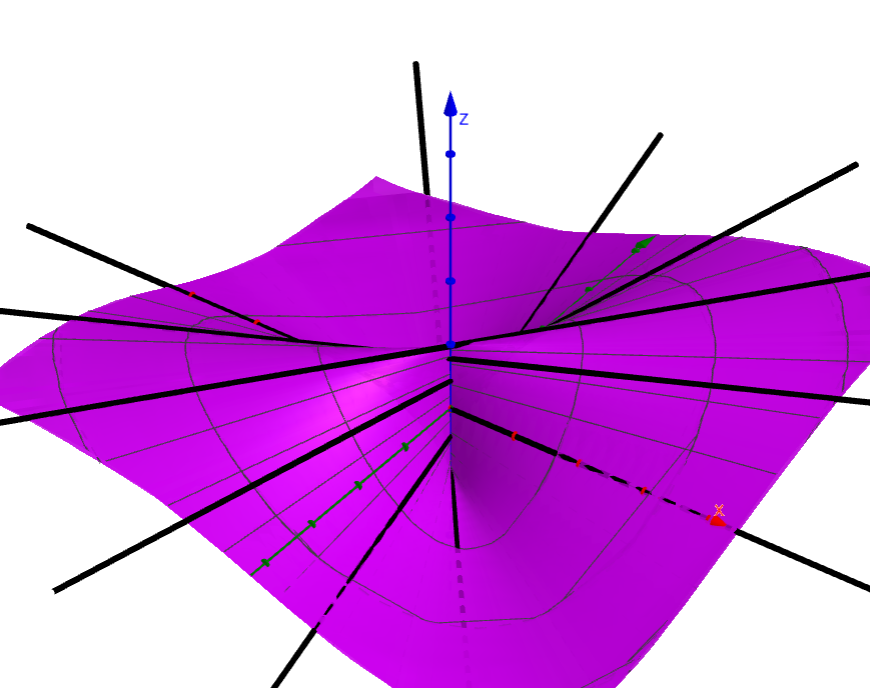
\includegraphics[width=7cm]{addchapters2/images/addchapters2_2025_02_21_2}
\end{wrapfigure}

\Ex $f(z) = \frac{1}{2i} \left(\frac{z}{\overline{z}} - \frac{\overline{z}}{z}\right) \qquad\qquad \letsymbol z = \rho e^{i\varphi}$

$f(z) = \frac{1}{2i} \left(\frac{\rho e^{i\varphi}}{\rho e^{-i\varphi}} - \frac{\rho e^{-i\varphi}}{\rho e^{i\varphi}}\right) =
\frac{1}{2i} \left(e^{2i\varphi} - e^{-2i\varphi}\right) = \frac{1}{2i} (\cos 2\varphi + i\sin 2\varphi - \cos 2\varphi + i\sin 2\varphi) = \sin 2\varphi$

Зафиксируем $\varphi = \varphi^* \in [0; 2\pi)$, тогда $\sin 2\varphi^* \in [-1; 1]$

$\lim_{z \to 0} f(z) = \lim_{\substack{\rho \to 0 \\ \varphi = \varphi^*}} f(z) = 
\lim_{\substack{\rho \to 0 \\ \varphi = \varphi^*}} \sin 2\varphi = \sin 2\varphi^* \in [-1; 1]$

Значения предела занимает отрезок $[-1; 1] \Longrightarrow \not\exists \lim_{z \to 0} f(z)$

На рисунке изображена $\sin 2\varphi$, на оси $Oz$ изображена $\RE w$. Черные линии - это возможные пути приближения $z$ к $0$

\Nota Путь следования предела аналогичен левостороннему и правостороннему пределами $\Real$-функций

\DefN{Непрерывность функций в точке $z_0$}

$f : D \longrightarrow G, z_0 \in D$, $f(z)$ называется непрерывной в $z_0$, если $\lim_{z \to z_0} f(z) = f(z_0)$

На языке приращений: $\Delta f = f(z_0 + \Delta z) - f(z_0) \underset{\Delta z \to 0}{\longrightarrow} 0$

$\Delta z = z - z_0 = \Delta x + i \Delta y \to 0 \Longrightarrow 
\begin{cases}\Delta x \to 0 \\ \Delta y \to 0\end{cases} \Longrightarrow 
\Delta \rho \to 0$

\subsubsection{3$^\circ$ Элементарные комплексные функции}

\ExN{1} Линейная $f(z) = az + b, \qquad\qquad a, b \in \Complex \quad a \neq 0$

Эта функция однозначная, однолистная $\Longrightarrow \exists f^{-1}(z) = g(z) = \frac{z - b}{a}$

\underline{Геометрический смысл}:

$a \in \Complex, z \in \Complex$

$az = |a| |z| (\cos (\varphi_a + \varphi_z) + i \sin (\varphi_a + \varphi_z))$ - поворот и растяжение 
($\varphi_a = \arg a$, $\varphi_z = \arg z$)

$az + b = (x_{az} + x_b) + i (y_{az} + y_b)$ - сдвиг

То есть линейная функция - композиция из поворота, растяжения и сдвига

\ExN{2} Степенная $w = z^n, \quad n \in \Natural$ - однозначная, может быть неоднолистной

Для $n \in \Rational$ функция становится неоднозначной

\Exs $w = z^2 \qquad\qquad z = \rho e^{i\varphi}, w = \rho^2 e^{2i\varphi}$

Пусть $z_1 \neq z_2$ и $w(z_1) = w(z_2)$, тогда $\arg z_1 = \arg z_2 \pm \pi$ 

$w(z_1) = \rho^2 e^{2i\arg z_1} = \rho^2 e^{2i (\arg z_1 + 2\pi k)}$

$w(z_2) = \rho^2 e^{2i\arg z_2} = \rho^2 e^{2i (\arg z_1 + \pi)} = \rho^2 e^{i (2\arg z_1 + 2\pi)} = w(z_1)$

Область однолистности $z^2$ - множество точек, для которых $\arg z \in [0; \pi)$

Точку $w = 0$ называют точкой разветвления

% https://www.geogebra.org/calculator/phuam9sh

\begin{wrapfigure}{r}{0pt}
    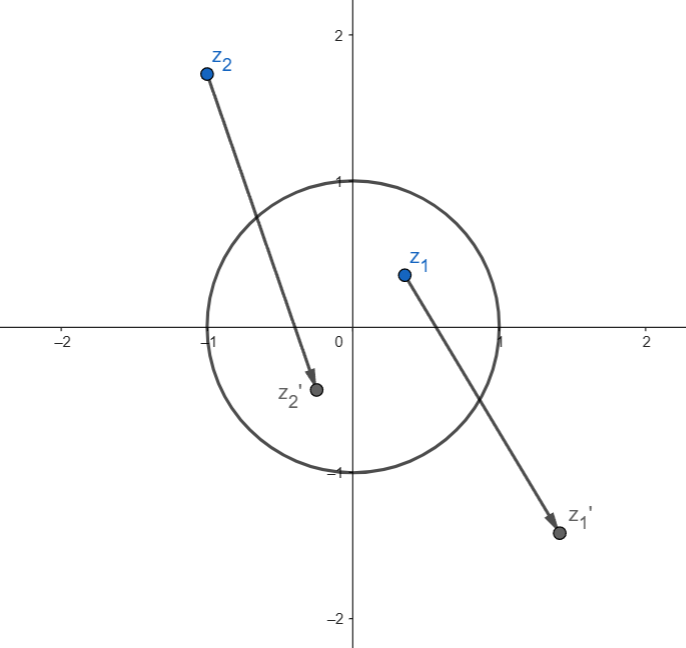
\includegraphics[width=7cm]{addchapters2/images/addchapters2_2025_02_21_1}
\end{wrapfigure}

\Exs $w = z^{-1} = \frac{1}{z} \qquad\qquad w(0) = \infty, w(\infty) = 0$

$z \in \Complex \setminus \{0\}$ - функция обратима

$w = re^{i\psi} = \frac{1}{\rho e^{i\phi}} = \frac{1}{\rho} e^{-i\varphi} \Longrightarrow |w| = \frac{1}{|z|}, \arg w = -\arg z$

Преобразование $|w| = \frac{1}{|z|}$ называется инверсией, а $\arg w = -\arg z$ дает симметрию относительно $\RE z$

\ExN{3} Рациональная $f(z) = \frac{P_n(z)}{Q_m(z)}, \qquad\qquad n, m \in \Natural$

\ExN{4} Показательная $w = e^z = e^x \cdot e^{iy} = e^x (\cos y + i \sin y)$

\underline{Свойства}: 

\begin{enumerate}
    \item $e^{z_1 + z_2} = e^{z_1} \cdot e^{z_2}$
    \item $\left(e^{z_1}\right)^{z_2} = e^{z_1 z_2}$
    \item $e^{z + 2\pi i} = e^{z} \cdot e^{2\pi i} = e^z$ - показательная функция периодична с периодом $2\pi i$
\end{enumerate}

\ExN{5} Логарифмическая $w = \Ln z$

Если $e^w = e^{u + vi} = e^u (\cos v + i \sin v) = z = |z| e^{i\arg z}$, то $u = \ln |z|$, $v = \arg z + 2\pi k$

Тогда \fbox{$\Ln z = \ln |z| + i (\arg z + 2\pi k)$}

$\ln z = \Ln z$ при $k = 0$ - т. н. главное значение




% end addchapters2_2025_02_21.tex

% begin addchapters2_2025_03_07.tex





Заметим, что $w = e^z = e^x (\cos y + i \sin y)$ - многолистная функция, а $w = \Ln z = \ln \rho + i (\arg z + 2\pi k)$ - многозначная

\ExN{6} Тригонометрические и гиперболические

\begin{multicols}{2}
    \begin{center}
        $\sin z = \frac{e^{iz} - e^{-iz}}{2i}$

        $\cos z = \frac{e^{iz} + e^{-iz}}{2}$

        $\sh z = \frac{e^{z} - e^{-z}}{2}$

        $\ch z = \frac{e^{z} + e^{-z}}{2}$
    \end{center}
\end{multicols}

\Nota Рассмотрим уравнение $\sin z = A \in \Complex$

$\frac{e^{iz} - e^{-iz}}{2i} = A \Longrightarrow e^{2iz} - 2iAe^{iz} - 1 = 0$

При $t = e^{iz}$ получаем квадратное уравнение, у которого в $\Complex$ всегда будет два корня. 
Это значит, что в $\Complex$ $\sin$ и $\cos$ принимают любые значения (то есть $|\sin z| > 1$)

\subsubsection{4$^\circ$ Дифференцирование ФКП}

\Def $w = f(z), w : D \subset \Complex \longrightarrow \Complex, z_0 \in D$. \textbf{Производная} функции
$w(z_0)$ - это предел $\lim_{\Delta z \to 0} \frac{f(z_0 + \Delta z) - f(z_0)}{\Delta z} = \lim_{\Delta z \to 0} \frac{\Delta f}{\Delta z}$, 
если он существует и не зависит от пути $z \to z_0$

\Mem Дифференцирование $y = f(x)$:

\begin{tabular}{ll}
    В Ф$_1$П: & $\Delta y = f(x_0 + \Delta x) - f(x_0) \underset{A \in \Real}{=} A\Delta x + o(\Delta x)$ \\
    В Ф$_2$П: & $\Delta f = f(x_0 + \Delta x, y_0 + \Delta y) - f(x_0, y_0) = A\Delta x + B \Delta y + \alpha_1 + \alpha_2 = 
    \frac{\partial f}{\partial x} \Delta x + \frac{\partial f}{\partial y} \Delta y + o(\Delta x) + o(\Delta y)$
\end{tabular}

\Def $f(z)$ называется дифференцируемой в точке $z_0$, если $\exists f^\prime(z_0) \in \Complex$

\Defs Дифференцируемая в точке $z_0$ функция $w = f(z)$, производная $f^\prime(z_0)$ которой непрерывна в $z_0$,
называется аналитической (или аналитичной) функцией в $z_0$

\begin{MyTheorem}
    \Ths Критерий аналитичности (или Условие Коши-Римана)

    \begin{center}
        $f(x) = u(x, y) + i v(x, y)$ аналитична в точке $z_0 = x + iy$ 
        
        \rotatebox{90}{$\Longleftrightarrow$}
    
        $\exists \frac{\partial u}{\partial x}, \frac{\partial u}{\partial y}, \frac{\partial v}{\partial x}, \frac{\partial v}{\partial y}$ непрерывны в $z$ и
        $\begin{cases}\frac{\partial u}{\partial x} = \frac{\partial v}{\partial y} \\ \frac{\partial u}{\partial y} = -\frac{\partial v}{\partial x}\end{cases}$
    \end{center}

    Причем, $f^\prime(z) = u_x + i v_x = v_y - i u_y = u_x - i u_y = v_y + i v_x$
\end{MyTheorem}

\begin{MyProof}
    \fbox{\Longrightarrow} \ $f$ аналитическая в $z$ $\Longleftrightarrow \exists$ непрерывная 
    $f^\prime(z) = \\ = \lim_{\Delta z \to 0} \frac{\Delta f}{\Delta z} = [\text{предел не зависит от пути}] = 
    \lim_{\Delta x \to 0} \frac{f(x + \Delta x, y) - f(x, y)}{\Delta x} = \\
    = \lim_{\Delta x \to 0} \frac{u(x + \Delta x, y) + i v(x + \Delta x, y) - u(x, y) - v(x, y)}{\Delta x} = \\
    = \lim_{\Delta x \to 0} \left(\frac{u(x + \Delta x, y) - u(x, y)}{\Delta x} + i \frac{v(x + \Delta x, y) - v(x, y)}{\Delta x}\right) = \\
    = \lim_{\Delta x \to 0} \left(\frac{\Delta_x u}{\Delta x} + i \frac{\Delta_x v}{\Delta x}\right) = 
    \lim_{\Delta x \to 0} \frac{\Delta_x u}{\Delta x} + i \lim_{\Delta x \to 0} \frac{\Delta_x v}{\Delta x} = 
    \frac{\partial u}{\partial x} + i \frac{\partial v}{\partial x} = u_x + i v_x$

    Аналогично при $i \Delta y \to 0$ получаем $\lim_{\Delta y \to 0} \frac{f(x, y + \Delta y) - f(x, y)}{i \Delta y} = \\
    = \lim_{\Delta y \to 0} \left(\frac{u(x, y + \Delta y) - u(x, y)}{i \Delta y} + \frac{v(x, y + \Delta y) - v(x, y)}{\Delta y}\right) = 
    \lim_{\Delta y \to 0} \frac{\Delta_x v}{\Delta y} - i \lim_{\Delta y \to 0} \frac{\Delta_x u}{\Delta x} = 
    v_y - i u_y$

    Итак, $f^\prime(z) = u_x + i v_x = v_y + i u_y$

    Отсюда $u_x = v_y$ и $u_y = -v_x$

    \mediumvspace 

    \fbox{\Longleftarrow} \ $\exists$ непрерывные $u_x, u_y, v_x, v_y \Longleftrightarrow u(x, y), v(x, y)$ 
    дифференцируемы в $(x, y)$, тогда $\Delta u = u_x \Delta x + u_y \Delta y + \alpha_1 (x, y, \Delta x, \Delta y) + 
    \alpha_2 (x, y, \Delta x, \Delta y)$

    $\alpha_1 = o(\Delta \rho), \quad \Delta \rho = (\Delta x)^2 + (\Delta y)^2$

    $\Delta v = v_x \Delta x + v_y \Delta_y + \beta_1 + \beta_2$

    $\Delta f = u(x + \Delta x, y + \Delta y) + iv(x + \Delta x, y + \Delta y) - (u(x, y) + i v(x, y)) = 
    u_x \Delta x + u_y \Delta y + \alpha + i(v_x \Delta x + v_y \Delta y + \beta)$

    $\frac{\Delta f}{\Delta z} = \frac{u_x \Delta x + u_y \Delta y + i v_x \Delta x + i v_y \Delta y}{\Delta x + i \Delta y} + 
    \frac{\alpha + i \beta}{\Delta x + i \Delta y} = \frac{u_x(\Delta x + i \Delta y)}{\Delta x + i \Delta y} + 
    \frac{v_x(i \Delta x - \Delta y)}{\Delta x + i \Delta y} + \frac{\alpha + i\beta}{\Delta x + i \Delta y} = 
    u_x + v_x i + \frac{\alpha + i \beta}{\Delta x + i \Delta y}$

    Тогда $\lim_{\Delta z \to 0} \frac{\Delta f}{\Delta z} = 
    u_x + i v_x + \lim_{\substack{\Delta x \to 0 \\ \Delta y \to 0}} \frac{\alpha + i \beta}{\Delta x + i \Delta y} = 
    u_x + i v_x \Longleftrightarrow f^\prime = u_x + i v_y$, существует и непрерывна в $(x, y)$
\end{MyProof}

\Nota Используя Условие Коши-Римана, получим равенство $u_x + i v_x = v_y - i u_y = u_x - i u_y = v_y + i v_x$

\Notas Коши-Риман в ПСК:

\begin{cases}
    \frac{\partial u}{\partial \rho} = \frac{1}{\rho} \frac{\partial v}{\partial \varphi} \\
    \frac{\partial u}{\partial \varphi} = -\frac{1}{\rho} \frac{\partial v}{\partial \rho}
\end{cases}

Тогда $f^\prime(z) = \frac{1}{z} \left(\frac{\partial v}{\partial \varphi} - i \frac{\partial u}{\partial \varphi}\right) = \frac{\rho}{z} \left(\frac{\partial u}{\partial \rho} + i \frac{\partial v}{\partial \rho}\right)$

\begin{MyProof}
    $u_\rho = u_x \frac{\partial x}{\partial \rho} + u_y \frac{\partial y}{\partial \rho} = u_x \cos \varphi + u_y \sin \varphi$

    $v_\varphi = v_x \frac{\partial x}{\partial \varphi} + v_y \frac{\partial y}{\partial \varphi} = 
    -\rho v_x \sin \varphi + \rho v_y \cos \varphi = \rho u_y \sin \varphi + \rho u_x \cos \varphi = \rho u_\rho$

    \Lab $\frac{\partial u}{\partial \varphi} = -\frac{1}{\rho} \frac{\partial v}{\partial \rho}$
\end{MyProof}

\mediumvspace

\underline{Свойства аналитических функций}

Пусть $f, g$ - аналитические функции, тогда:

\begin{enumerate}[label=\arabic*$^\circ$]
    \item Линейность: $af + bg$ - аналитическая
    \item Композиция: $f(g(z))$ - аналитическая
    \item Произведение: $f \cdot g$ - аналитическая
\end{enumerate}

\Nota Доказательства свойств элементарные, все сводится к сведению к $u$ и $v$

\Ex $w = \frac{1}{z} = \frac{1}{x + iy} = \frac{x}{x^2 + y^2} - i \frac{y}{x^2 + y^2} = u(x, y) + i v(x, y)$

$u_x = \frac{x^2 + y^2 - 2x^2}{(x^2 + y^2)^2} = \frac{y^2 - x^2}{(x^2 + y^2)^2}$

$v_y = \frac{-x^2 - y^2 + 2y^2}{(x^2 + y^2)^2} = \frac{y^2 - x^2}{(x^2 + y^2)^2} = u_x$

$u_y = \frac{-2xy}{(x^2 + y^2)^2}$

$v_x = \frac{2xy}{(x^2 + y^2)^2} = -u_y$

Таким образом, $\frac{1}{z}$ - аналитическая функция

\Ex $w = \overline{z} = x - iy$

$u_x = 1$, $v_y = -1 \neq u_x$ - не аналитическая функция



% end addchapters2_2025_03_07.tex



\end{document}

